\documentclass{article}

%packages
\usepackage[LGR]{fontenc}
\usepackage[english,greek]{babel}
\usepackage{amsfonts}
\usepackage{amsmath}
\usepackage{graphicx}
\usepackage{polynom}
\usepackage{hyperref}

\hypersetup{
    colorlinks = true,
    linkcolor  = blue,
    filecolor  = blue,      
    urlcolor   = blue,
}

%commands
\newcommand{\blank}[1]{\hspace*{#1}}
\newcommand{\myspace}{\blank{0.3cm}}
\newcommand{\lt}[1]{\latintext #1\greektext}
\newcommand{\gt}[1]{\greektext #1\latintext}
\newcommand{\task}[2]{\newpage\section*{Άσκηση #1:\\#2}}
\newcommand{\xor}[2]{$#1 \oplus #2$}
\newcommand{\xorthr}[3]{$#1 \oplus #2 \oplus #3$}
\newcommand{\myline}[3]{\hline $#1$ & $#2$ & $#3$ & \xorthr{#1}{#2}{#3}\\}
\newcommand{\myotherline}[6]{\hline (#1) #2 : #3 & (#4) #5 : #6\\}
\newcommand{\blt}[1]{\lt{\textbf{#1}}}
\newcommand{\ltext}[1]{\text{\lt{#1}}}

%default parameters
\setcounter{MaxMatrixCols}{20}
\setlength{\parindent}{0pt}

%info
\title{\textbf{\huge \lt{Project I}\\ Συμμετρική Κρυπτογραφία}}
\author{\LARGE Ασημάκης Κύδρος \\ \LARGE ΑΕΜ: 3881 \\ \LARGE \lt{asimakis@csd.auth.gr}}
\date{\LARGE \today}

\begin{document}
\Large
\maketitle

\task{1}{
    Το μήνυμα \textit{''οκηθμφδζθγοθχυκχσφθμφμχγ''} έχει κρυπτογραφηθεί με τον παρακάτω αλγόριθμο:
    \begin{center}
        \textit{\normalsize Κάθε γράμμα του αρχικού μηνύματος αντικαθίσταται με την αριθμητική του τιμή ($\alpha \rightarrow 1, \beta \rightarrow 2, ... , \omega \rightarrow 24$), η οποία μετέπειτα προσθέτεται με την τιμή $f(x_0)$ του πολυωνύμου $f(x) = x^5 + 3x^3 + 7x^2 + 3x^4 + 5x + 4$, όπου $x_0$ μια ρίζα του πολυωνύμου $g(x) = x^2 + 3x + 1$. Το αποτέλεσμα αντικαθίσταται με το πλέον αντίστοιχο γράμμα.}
    \end{center}
    Αποκρυπτογραφήστε το.
}

Λύνοντας το $g(x)$ με διακρίνουσα καταλήγουμε στις ρίζες
\begin{equation*}
    x_0 = -1 - \phi,\myspace  x_0' = -1 - \bar{\phi}
\end{equation*}
όπου $\phi$ η χρυσή τομή. Άρρητες τιμές άρα η προσέγγιση αυτή δεν είναι ιδανική.\\

Κάνουμε διαίρεση πολυωνύμων μεταξύ των $f(x), g(x)$:

\begin{equation*}
         \polylongdiv[style=D]{x^5 + 3x^4 + 3x^3 + 7x^2 + 5x + 4}{x^2 + 3x + 1}
\end{equation*}
    
Επομένως ισχύει γενικά πως $f(x) = (x^3 + 2x + 1)g(x) + 3$. Άρα $f(x_0) = 3$,
δηλαδή η κρυπτογράφηση εν τέλη χρησιμοποιεί το \textbf{κρυπτοσύστημα του Καίσαρα}.

\newpage
Για να αποκρυπτογραφήσουμε το μήνυμα αντικαθιστούμε κάθε γράμμα με το γράμμα τρεις θέσεις πριν από αυτό.\\ Εφαρμόζοντάς το αυτό ανακαλύπτουμε ότι το αρχικό μήνυμα ήταν

\begin{center}
    \textit{\textbf{ μηδεισ αγεωμετρητοσ εισιτω}}
\end{center}
το οποίο ήταν η επιγραφή στην είσοδο της Ακαδημίας του Πλάτωνα.\\

Στο \lt{task 1.py} υλοποιείται ακριβώς η παραπάνω διαδικασία, και επιβεβαιώνει το αποτέλεσμα.

\task{2}{
    Αποκρυπτογραφήστε τα κείμενα που βρίσκονται στο \lt{github} και κρυπτογραφήθηκαν με τον αλγόριθμο του \lt{Vigen\`ere}. Βρείτε το μήκος του κλειδιού εφαρμόζοντας \lt{test Kasiski} ή μέθοδο \lt{Friedman}.
}

Έστω το κάθε κρυπτοκείμενο είναι της μορφής $c_1c_2\cdot\cdot\cdot c_k$.\\

Βρίσκουμε το (πιθανό) μήκος του κάθε κλειδιού εφαρμόζοντας το τεστ του \lt{Friedman}: ξεκινάμε υποθέτοντας μήκος\\ $\rho$ = 2 και τρέχοντας τις παρακάτω λέξεις
\begin{align*}
    C_1 &= [c_1, c_{1+\rho}, ...]\\
    C_2 &= [c_2, c_{2+\rho}, ...]\\
    .\\
    .\\
    .\\
    C_\rho &= [c_\rho, c_{2\rho}, ...]
\end{align*}
υπό το τεστ
\begin{equation*}
    IC(C_i) \approx^? 0.0665
\end{equation*}
όπου
\begin{equation*}
    IC = \frac{\sum_{i = 1}^{26}m_i^2}{k^2}
\end{equation*}
με $m_i$ το πλήθος εμφανίσεων του \lt{i}-οστού γράμματος του αλφαβήτου στην λέξη.\\

Επαναλαμβάνουμε το παραπάνω για όλα τα $\rho$ μέχρι κάποιο να περάσει το τεστ ή να φτάσουμε το μήκος του κρυπτογράμματος (το κλειδί δεν θα είναι ποτέ τόσο μεγάλο).\\

Τρέχοντας το παραπάνω για τα δύο κρυπτομηνύματα παίρνουμε (πιθανό) μήκος κλειδιού 7 και για τα δύο. Έχοντας τα μήκη των κλειδιών, μπορούμε να τα προσεγγίσουμε. Κάνουμε συχνοτική ανάλυση σε κάθε κρυπτόγραμμα, χωρίζοντάς το σε 7 (όσα και το μήκος του κλειδιού) υπό-μηνύματα με τέτοιον τρόπο ώστε κάθε γράμμα του δωθέν υπο-μηνύματος να κρυπτογραφήθηκε με το ίδιο γράμμα του κλειδιού. Κατ' αυτόν τον τρόπο, τα υπό-μηνύματα είναι σαν να είναι κρυπτογράμματα κρυπτογράφησης του Καίσαρα.\\

Εφόσον για κάθε υπο-μήνυμα το κλειδί-κομμάτι είναι\\ στανταρ, ψάχνουμε σε καθένα το πιο συχνό γράμμα. Στοιχιματίζουμε πως αυτό θα αντιστοιχεί σε κάποιο από τα πιο συχνά γράμματα του αγγλικού αλφαβήτου, δηλαδή στο \textbf{E} ή \textbf{T}. Δημιουργούμε μια λέξη με όλα αυτά τα γράμματα.\\

Αξιοποιούμε το παραπάνω στοίχημα αποκρυπτογραφόντας τις προαναφαιρόμενες 2 λέξεις με κάθε συνδυασμό στο $\{E, T\}^7$. Κάποιο από τα αποτελέσματα της αποκρυπτογράφησης είναι το κλειδί ή το προσεγγίζει αρκετά, και  βλέποντάς τα μπορούμε πιθανώς να τα προσεγγίσουμε.\\

Για το πρώτο κείμενο είναι αρκετά προφανές ότι το κλειδί είναι η λέξη \textit{\blt{EMPEROR}}, διότι υπάρχει στις περιπτώσεις, όλες οι υπόλοιπες το προσεγγίζουν και επίσης αποκρυπτογραφεί το κείμενο τέλεια.\\

\newpage

Για το δεύτερο δεν είμαστε τόσο τυχεροί, αλλά\\ παρατηρούμε πως οι λέξεις \blt{SLANNON} και \blt{SWANNON} που υπάρχουν στις περιπτώσεις παράγουν αποκρυπτογράφηση που βγάζει αρκετό νόημα, και όλες οι υπόλοιπες φαίνεται να τα προσεγγίζουν. Μπορούμε επομένως να μαντέψουμε, και από την μερική αποκρυπτογράφηση, ότι το δεύτερο κλειδί είναι η λέξη \textit{\blt{SHANNON}}, και όντως αυτή αποκρυπτογραφεί το κείμενο τέλεια.\\

Η υλοποίηση του παραπάνω μπορεί να βρεθεί στο \lt{task 2.py} και τα αποτελέσματα της αποκρυπτογράφησης στο\\ \lt{task 2 results.txt}. Το πρώτο είναι ο λόγος του \lt{Charlie Chaplin} στο φινάλε του \textit{\lt{The Great Dictator}}. Το\\ δεύτερο είναι απόσπασμα από τον λόγο \textit{\lt{Creative Thinking}} του \lt{Claude Shannon}.

\task{3}{
    Έστω \lt{m} ένα \lt{16-bit} μήνυμα που\\ κρυπτογραφείται σε \lt{c} με τον εξής τρόπο:
    \[c = m \oplus (m << 6) \oplus (m << 10)\]
    Βρείτε τον γενικό τύπο αποκωδικοποίησης και υλοποιείστε τον σε κώδικα.
}

Έστω ότι 
\begin{align*}
    m &= M_{0}M_{1}M_{2}M_{3}M_{4}M_{5}M_{6}M_{7}M_{8}M_{9}M_{10}M_{11}M_{12}M_{13}M_{14}M_{15}\\
    c &= C_{0}C_{1}C_{2}C_{3}C_{4}C_{5}C_{6}C_{7}C_{8}C_{9}C_{10}C_{11}C_{12}C_{13}C_{14}C_{15}    
\end{align*}
όπου $M,C$ \lt{bits}. Ισχύουν τα παρακάτω:
\begin{center}
    \begin{tabular}{|c|c|c|c|}
        \hline
        $m$ & $m << 6$ & $m << 10$ & $c$\\
        \myline{M_{0}}{M_{6}}{M_{10}}
        \myline{M_{1}}{M_{7}}{M_{11}}
        \myline{M_{2}}{M_{8}}{M_{12}}
        \myline{M_{3}}{M_{9}}{M_{13}}
        \myline{M_{4}}{M_{10}}{M_{14}}
        \myline{M_{5}}{M_{11}}{M_{15}}
        \myline{M_{6}}{M_{12}}{M_{0}}
        \myline{M_{7}}{M_{13}}{M_{1}}
        \myline{M_{8}}{M_{14}}{M_{2}}
        \myline{M_{9}}{M_{15}}{M_{3}}
        \myline{M_{10}}{M_{0}}{M_{4}}
        \myline{M_{11}}{M_{1}}{M_{5}}
        \myline{M_{12}}{M_{2}}{M_{6}}
        \myline{M_{13}}{M_{3}}{M_{7}}
        \myline{M_{14}}{M_{4}}{M_{8}}
        \myline{M_{15}}{M_{5}}{M_{9}}
        \hline
    \end{tabular}
\end{center}

Παρατηρούμε πως το κρυπτόγραμμα $c$ κουβαλάει το ίδιο όλη την απαραίτητη πληροφορία για την αποκρυπτογράφησή του.

Παρατηρούμε επίσης πώς
\begin{align*}
    M_6 &= C_2 \oplus C_4 \oplus C_6 \oplus C_8 \oplus C_{10}\\
    M_5 &= C_1 \oplus C_3 \oplus C_5 \oplus C_7 \oplus C_9
\end{align*}

Με το μάτι επιβεβαιώνουμε πως η παραπάνω σχέση\\ γενικεύεται, αν σκεφτούμε το \lt{bitstream} του κρυπτογράμματος ως ''κορδέλα''.\\

Επομένως συνεπάγουμε πως:
\begin{align*}
    m &= (M_i : i\in[0, 15]) \ni\\
    M_i &= C_{i -_{16} 4} \oplus C_{i -_{16} 2} \oplus C_i \oplus C_{i +_{16} 2} \oplus C_{i +_{16} 4}
\end{align*}
όπου $-_{16}, +_{16}$ οι αντίστοιχες πράξεις $mod 16$.\\

Η παραπάνω διαδικασία υλοποιείται ολόιδια στο \lt{task 3.py}.
Τρέχοντας το τεστ της \lt{main} βλέπουμε πως το \lt{original\\ plaintext} και το αποτέλεσμα της αποκρυπτογράφησης\\ ταυτίζονται.

\task{4}{
    Να αποδείξετε ότι, αν στο σύστημα μετατόπισης διαλέγουμε τυχαία τα κλειδιά από το σύνολο $\{0, 1, ..., 23\}$, τότε το σύστημα έχει τέλεια ασφάλεια.
}

Όντως, αν για κάθε γράμμα του \lt{plaintext} διαλέγουμε ένα κλειδί ομοιόμορφα στην τύχη τότε το σύστημα γίνεται\\ τελείως ασφαλές, και αυτό φαίνεται από 2 πράγματα:
\begin{enumerate}
    \item αναλύσεις κρυπτογραμμάτων με οποιαδήποτε μετρική, όπως συχνότητα γραμμάτων, χάνουν την ουσία τους, και
    \item το συνολικό κλειδί θα έχει μήκος ίσο με το \lt{plaintext}, και άρα μέσω του θεωρήματος του \lt{Shannon} το σύστημα πρέπει να έχει τέλεια ασφάλεια.
\end{enumerate}

\task{5}{
    Υλοποιήστε τον \lt{OTP}, μετατρέποντας εσωτερικώς το δωσμένο \lt{plaintext} σε \lt{bits} βάσει του παρακάτω πίνακα. Να δουλεύει και η κρυπτογράφηση και η αποκρυπτογράφηση και κάθε αποτέλεσμα να είναι σε \lt{text}, όχι \lt{bits}.
}

\begin{center}
    \lt{\begin{tabular}{|c||c|}
        \myotherline {0}{A}{00000}{16}{Q}{10000}
        \myotherline {1}{B}{00001}{17}{R}{10001}
        \myotherline {2}{C}{00010}{18}{S}{10010}
        \myotherline {3}{D}{00011}{19}{T}{10011}
        \myotherline {4}{E}{00100}{20}{U}{10100}
        \myotherline {5}{F}{00101}{21}{V}{10101}
        \myotherline {6}{G}{00110}{22}{W}{10110}
        \myotherline {7}{H}{00111}{23}{X}{10111}
        \myotherline {8}{I}{01000}{24}{Y}{11000}
        \myotherline {9}{J}{01001}{25}{Z}{11001}
        \myotherline{10}{K}{01010}{26}{.}{11010}
        \myotherline{11}{L}{01011}{27}{!}{11011}
        \myotherline{12}{M}{01100}{28}{?}{11100}
        \myotherline{13}{N}{01101}{29}{(}{11101}
        \myotherline{14}{O}{01110}{30}{)}{11110}
        \myotherline{15}{P}{01111}{31}{-}{11111}
        \hline
    \end{tabular}}
\end{center}

\hfill\\

Υλοποιούμε το Σημειωματάριο Μιας Φοράς όπως μας καθοδηγεί η θεωρία: η συνάρτηση δέχεται το \lt{plaintext} σε μορφή κειμένου, και ενδεχομένως ένα κλειδί σε \lt{bits}. Μετατρέπουμε το κείμενο-μήνυμα στα \lt{bits} του για να ξέρουμε το πλήθος τους και προχωράμε στο κλειδί. Αν δεν δώθηκε ένα τότε δημιουργούμε ένα άλλο (ψεύδο)τυχαία.\\

Εκτελούμε \lt{bitwise xor} το κλειδί με τα \lt{bits} του \lt{plaintext} και, βάσει του ανιστρόφου του αρχικού πίνακα, μετατρέπουμε το αποτέλεσμα σε κείμενο. Επιστρέφουμε το κλειδί και το κρυπτόγραμμα.\\

Τρέχοντας το \lt{test} της \lt{main} επιβεβαιωνόμαστε πως η υλοποίηση είναι σωστή. Προφανώς, ο \lt{OTP} είναι και ο ίδιος του ο \lt{decryptor}. Απλά απαιτείται να δωθεί το σωστό κλειδί.\\

Η υλοποίηση δίνεται από το \lt{task 5.py}.

\task{6}{
    Βρείτε το πλήθος των ανάγωγων πολυωνύμων βαθμού 10 στο σώμα $\mathbb{F}_2$, αν αυτό δίνεται από τον εξής τύπο
    \[N_2(n) = \frac{1}{n}\sum_{d|n}\mu(d)2^{n/d}, \myspace n: \myspace degree\]
    όπου
    \[
        \mu(d) = 
        \begin{cases}
            1,      &d = 1\\
            (-1)^k, &d = p_1p_2....p_k \myspace (p_i \myspace primes)\\
            0,      &otherwise
        \end{cases}
    \]
}

Έχουμε
\begin{equation}
    N_2(10) = \frac{1}{10}\sum_{d|10}\mu(d)2^{10/d}
\end{equation}

Οι διαιρέτες του 10 είναι \{1, 2, 5, 10\}. Επομένως η (1) γίνεται
\begin{equation}
    N_2(10) = \frac{1}{10}(\mu(1)2^{10} + \mu(2)2^5 + \mu(5)2^2 + \mu(10)2)
\end{equation}

Εξ' ορισμού της $\mu$ ισχύουν τα εξής:
\begin{align*}
    \mu(1) &= +1\\
    2 \myspace prime \Rightarrow k = 1 \Rightarrow  \mu(2) &= -1\\
    5 \myspace prime \Rightarrow k = 1 \Rightarrow  \mu(5) &= -1\\
    10 = 2\cdot5     \Rightarrow k = 2 \Rightarrow  \mu(10) &= +1
\end{align*}

\newpage
Βάσει των παραπάνω, η (2) γίνεται
\begin{equation*}
    N_2(10) = \frac{1}{10}(2^{10} - 2^5 - 2^2 + 2) = \frac{1}{10}\cdot990 = 99
\end{equation*}

Η παραπάνω λύση υλοποιείται ολόιδια στο \lt{task 6.py} αλλά και στο \lt{task 6.sage}, όπως ζητείται.\\ Για την εύρεση των πρώτων παραγόντων χρησιμοποιείται\\ η \lt{trial\_division} των σημειώσεων.

\task{7}{
    Υλοποιήστε τον \lt{RC4} και, χρησιμοποιώντας το κλειδί \textit{\lt{\large'HOUSE'}} \Large κρυπτογραφήστε το μήνυμα\\
    \textit{\lt{\normalsize'MISTAKESAREASSERIOUSASTHERESULTSTHEYCAUSE'}}\\
    \Large Η υλοποίηση να αποκρυπτογραφεί σωστά.\\ Χρησιμοποιήστε τον πίνακα της άσκησης 5.
}

Δεχόμαστε το \lt{plaintext} και το κλειδί σε μορφή κειμένου. Μετατρέπουμε και τα δύο σε ακολουθίες ακεραίων με βάση τον δεδομένο πίνακα και περνάμε ως \lt{seed} στον \lt{scheduler} τη μετάφραση του κλειδιού.\\

Η υλοποίηση του δρομολογητή και της κλειδορροής\\ ακολουθούν πιστά τη θεωρία, με μόνες αλλαγές ότι η\\ κλειδορροή επιστρέφεται ολάκερη, όχι κομμάτι-κομμάτι, και κάθε κομμάτι είναι των 5 \lt{bit} για να ταιρίαζει με τον δωσμένο πίνακα μετάφρασης.\\

Τέλος εκτελούμε \lt{byte-wise xor} την κλειδορροή με τους κωδικούς-μετάφραση του \lt{plaintext} και μετατρέπουμε το\\ αποτέλεσμα σε κείμενο για να σχηματίσουμε το \lt{ciphertext}.\\

Τρέχοντας το \lt{test} της \lt{main} επιβεβαιωνόμαστε πως και η κρυπτογράφηση και η αποκρυπτογράφηση έγιναν σωστά.\\ Παρατηρούμε πως το κλειδί \lt{'HOUSE'} επιστρέφει πάντα την ίδια κρυπτογράφηση, καθώς και πως ο \lt{RC4} αποκρυπτογραφεί τον εαυτό του με το σωστό κλειδί.\\ Και τα δύο αναμενόμενα καθώς αποτελεί ντετερμινιστική\\ παραλλαγή του \lt{one time pad}.\\

Η υλοποίηση δίνεται από το \lt{task 7.py}.


\task{8}{
    Υπολογίστε την διαφορική ομοιομορφία\\ (\lt{differential uniformity}):
    \lt{\large\[
        Diff(S) = \max_{\textbf{x}\in\{0,1\}^6-\{\textbf{0}\},\textbf{y}\in\{0,1\}^4}|\{\textbf{z}\in\{0,1\}^6\ni S(\textbf{z} \oplus \textbf{x}) \oplus S(\textbf{z}) = \textbf{y}\}|
    \]}
    \Large του \lt{S-box S}: 
}
\begin{equation*}
    \large
    \begin{bmatrix}
        0 & 2 & 3 & 7 & 9 & 12 & 15 & 7 & 6 & 15 & 15 & 1 & 7 & 3 & 1 & 0 \\
        1 & 5 & 6 & 13 & 4 & 1 & 5 & 11 & 7 & 8 & 7 & 1 & 1 & 3 & 2 & 13 \\
        5 & 3 & 5 & 12 & 11 & 1 & 1 & 5 & 13 & 0 & 15 & 7 & 2 & 2 & 13 & 0 \\
        3 & 12 & 3 & 11 & 2 & 2 & 2 & 4 & 6 & 5 & 5 & 0 & 4 & 3 & 1 & 0
    \end{bmatrix}    
\end{equation*}

\hfill\\

Η λύση δίνεται από το \lt{task 8.py}. Η θεωρία ορίζει πως η \lt{S} τιμή του \lt{6-bit} αριθμού $X_0X_1X_2X_3X_4X_5$ δίνεται από την \lt{4-bit} τιμή που βρίσκεται στο κιβώτιο στη θέση
\begin{equation*}
    row = (X_0X_5)_{10}, \myspace col = (X_1X_2X_3X_4)_{10}
\end{equation*}

Η συνάρτηση \lt{coords} υλοποιεί ακριβώς αυτό και επιστρέφει τις παραπάνω τιμές.\\

Έχοντας τις συντεταγμένες των \blt{z}, \blt{z} $\oplus$ \blt{x}, κάνουμε \lt{bitwise xor} τις αντίστοιχες τιμές και συγκρίνουμε το αποτέλεσμα με το \blt{y}. Αποθηκεύουμε το πλήθος των \blt{z} που ικανοποιούν την παραπάνω ισότητα στη μεταβλητή \blt{norm}.\\

Τρέχουμε την παραπάνω διαδικασία για όλα τα πιθανά \blt{z} κόντρα σε κάθε πιθανό ζεύγος (\blt{x}, \blt{y}) του $\{0,1\}^6 - \{000000\} \times \{0,1\}^4$. Η μέγιστη τιμή όλων των \blt{norm} είναι και η ζητούμενη λύση.
Για το δεδομένο κιβώτιο βγαίνει πως
\begin{equation*}
    Diff(S) = 14
\end{equation*}

\task{9}{
    Εξετάστε αν ισχύει το \lt{avalanche effect} στον \lt{AES-128} φτιάχνοντας πολλά ($>$30) ζευγάρια μηνυμάτων που διαφέρουν σε ένα \lt{bit} και\\ μετρώντας σε πόσα \lt{bits} διαφέρουν τα\\ αντίστοιχα κρυπτομηνύματα. Δοκιμάστε με δύο καταστάσεις λειτουργίας (\lt{ECB} και \lt{CBC}) και χρησιμοποιώντας μήκος μηνυμάτων 2\\ \lt{block} (δηλαδή 256-\lt{bit}).
}

Η λύση δίνεται από το \lt{task 9.py}. Για τη σωστή λειτουργία του προγράμματος απαιτείται το πακέτο \lt{pycryptodome} το οποίο μπορεί να εγκατασταθεί επικαλώντας το \lt{pip install pycryptodome} στη γραμμή εντολών. Υπάρχει περίπτωση η εγκατάσταση να κάνει \lt{conflict} με το παλιό και πλέον \lt{deprecated} πακέτο \lt{PyCrypto}, σε περίπτωση που αυτό είναι ήδη εγκαταστημένο. Σε αυτή τη περίπτωση πρέπει πρώτα να\\ απεγκατασταθεί το \lt{PyCrypto} επικαλώντας το \lt{pip uninstall PyCrypto}.\\

Αρχικά δημιουργούμε 100 μηνύματα, χρησιμοποιώντας κάθε φορά το τελευταίο μήνυμα της λίστας και αλλάζοντας ένα τυχαίο \lt{bit} από αυτό για να προκύψει ένα καινούριο μήνυμα. Το υλοποιούμε έτσι ώστε, στη λίστα, κάθε στοιχείο να έχει ''γείτονες'' δύο αριθμούς που διαφέρουν από αυτό ακριβώς σε ένα \lt{bit}, ώστε η περαιτέρω δουλειά να είναι ενστικτώδης.\\

\newpage

Δημιουργούμε δύο \lt{ciphers}, ένα για κάθε κατάσταση λειτουργίας, και τρέχουμε και για τα δύο το εξής τεστ: Κρυπτογραφούμε δύο γείτονες και κάνουμε \lt{xor} τα αντίστοιχα κρυπτομηνύματα. Το πλήθος των άσσων στο αποτέλεσμα δείχνει σε πόσα \lt{bits} διαφέρουν τα δύο κρυπτομηνύματα (εξ' ορισμού της \lt{xor}). Αποθηκεύουμε το άθροισμα αυτών των πληθών για τα 100 ζεύγη και το επιστρέφουμε ως ποσοστό.\\

Παρατηρούμε πως, για κατάσταση λειτουργίας \lt{ECB}, ο \lt{AES} σκοράρει πολύ άσχημα· είναι γνωστό πως το \lt{ECB-mode} δεν πρέπει να χρησιμοποιείται για πολλούς λόγους. Αντιθέτως, για \lt{CBC} ο \lt{AES} σκοράρει κοντά στο 50\%, επομένως ισχύει το \lt{avalanche effect}.

\task{10}{
    Ανοίξτε το \lt{secure.zip} με τη βοήθεια του εισαγωγικού \lt{pdf}.
}

Περνάμε το \lt{pdf} από έναν \lt{online pdf metadata extractor}, εγώ χρησιμοποίησα \href{https://products.groupdocs.app/metadata/export/pdf}{αυτόν}. Στα \lt{metadata} θα βρούμε ένα \lt{string} που μοίαζει να είναι κωδικοποιημένο σε \lt{Base64}:
\begin{center}
    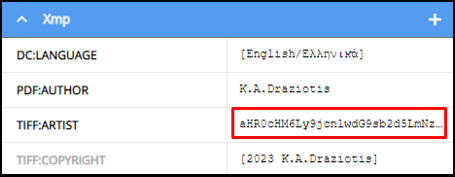
\includegraphics[scale=1]{files/pdf_metadata.png}
\end{center}
Το \lt{string} αυτό είναι το
\begin{center}
    \small
    \lt{aHR0cHM6Ly9jcnlwdG9sb2d5LmNzZC5hdXRoLmdyOjgwODAvaG9tZS9wdWIvMTUv}
\end{center}
και η αποκωδικοποίησή του από \lt{Base64}, οποία έγινε με το \href{https://www.base64decode.org}{εξής} \lt{online tool}, δίνει το παρακάτω \lt{link}:
\begin{center}
    \lt{https://cryptology.csd.auth.gr:8080/home/pub/15/}
\end{center}
Αυτό το \lt{link} μας οδηγεί σε ένα \lt{custom sage site}, το οποίο μας πληροφορεί ότι ο \lt{Walter White} βρήκε το εξής μήνυμα στο εργαστήριό του, μια συνηθισμένη μέρα παραγωγής μπλε μεθαμφεταμίνης:
\begin{center}
    \lt{\#2-75-22-6!}
\end{center}

\newpage

Ο \lt{Walter White} ήταν χημικός, επομένως κάτι έχει να κάνει με χημεία το παραπάνω. Θεωρώντας τα νούμερα ατομικούς αριθμούς, παίρνουμε τα εξής στοιχεία:
\begin{align*}
    2 &\rightarrow \ltext{Helium (He)}\\
    75 &\rightarrow \ltext{Rhenium (Re)}\\
    22 &\rightarrow \ltext{Titanium (Ti)}\\
    6 &\rightarrow \ltext{Carbon (C)}
\end{align*}
άρα το \lt{password} είναι κάποια εκδοχή του \lt{\#HeReTiC!}, συγκεκριμένα το
\begin{center}
    \lt{\#heretic!}
\end{center}

Το άνοιγμα του \lt{secret.txt} μας οδηγεί στην εύρεση του κωδικού του \lt{secret2.zip}. Το \lt{block} που μας δίνεται ως \lt{hint} είναι ξανά κωδικοποιημένο σε \lt{Base64}, και η αποκωδικοποίησή του μας δίνει το \lt{decoded\_hint.txt}. Μέσα σε αυτό, μεταξύ άλλων, υπάρχει και ένα κομμάτι \lt{HTML} κώδικα. Τρέχοντάς τον χρησιμοποιώντας \href{https://onecompiler.com/html}{κάποιο} \lt{online tool} οδηγούμαστε στο εξής \lt{wall of text}:
\begin{center}
    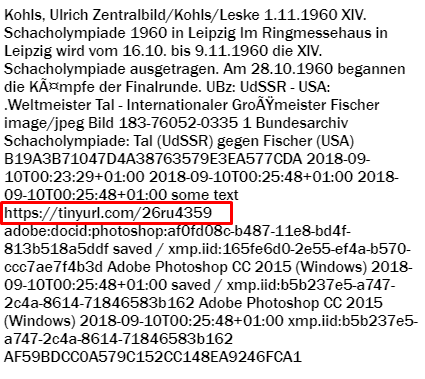
\includegraphics[scale=0.6]{files/tal_fischer_final_1960.png}
\end{center}

\newpage

Αυτό το κείμενο αφορά την παρακάτω φωτογραφία, που βγήκε στην Σκακιστική Ολυμπιάδα της Λειψίας του 1960 μεταξύ των \lt{Bobby Fischer} και \lt{Mikhail Tal}:
\begin{center}
    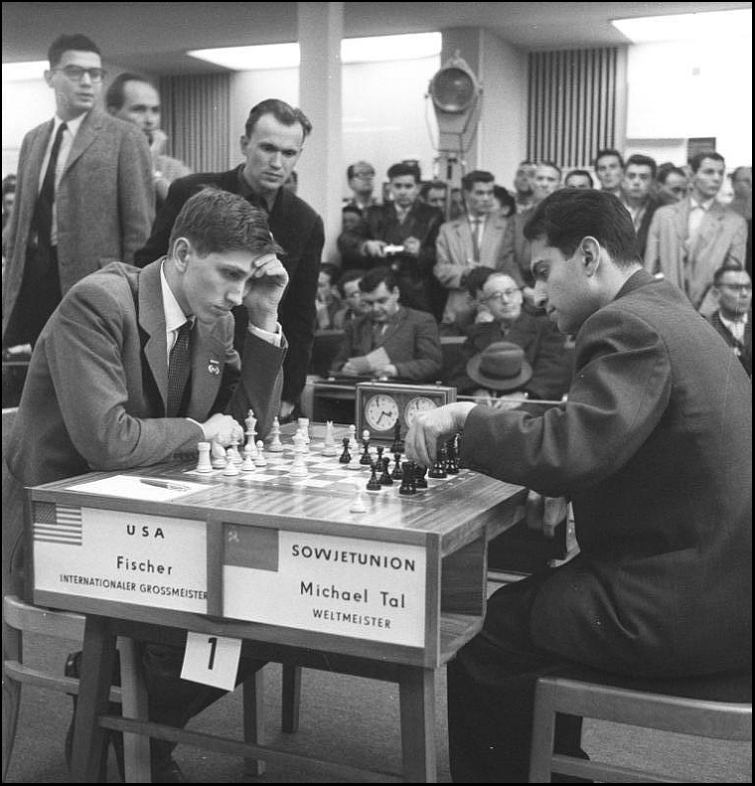
\includegraphics[scale=0.5]{files/bobby_vs_misha.png}\\
    \lt{\large(photo by German photographer Ulrich Kohls)}
\end{center}

\newpage

Εμάς μας ενδιαφέρει το \lt{link} που φαίνεται υπογραμμισμένο, το οποίο μας οδηγεί σε ένα καινούριο \lt{custom sage site} που μας προκαλεί να κερδίσουμε την παρακάτω παρτίδα σκάκι ως λευκά:
\begin{center}
    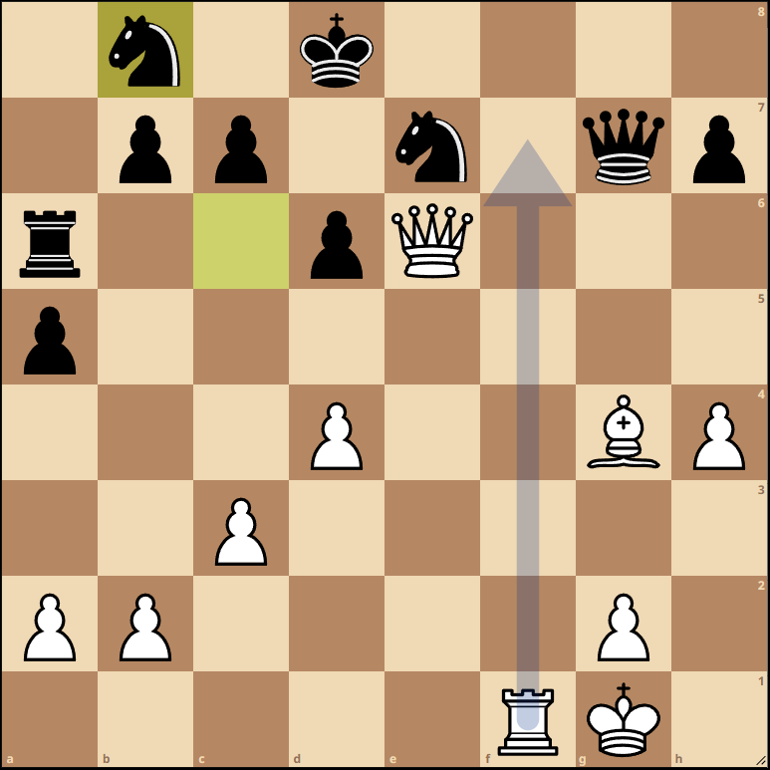
\includegraphics[scale=0.5]{files/chessgame.png}
\end{center}

Το \lt{stockfish 15} δίνει την κίνηση που φαίνεται ως την\\ καλύτερη, κοινώς την
\blt{Rf7}. Το \lt{site} μας καθοδηγεί να την κάνουμε \lt{hash} με \lt{MD5} για να ανοίξουμε το \lt{zip}, και όντως το
\begin{center}
    \lt{f1f5e44313a1b684f1f7e8eddec4fcb0}
\end{center}
λειτουργεί ως κλειδί και αποκαλύπτει το πιστοποιητικό-\lt{hash}:
\begin{center}
    \blt{\textit{be121740bf988b2225a313fa1f107ca1}}
\end{center}
\end{document}
